\section{Interface Iteration}\label{interface-iteration}

\begin{figure}[htbp]
\centering
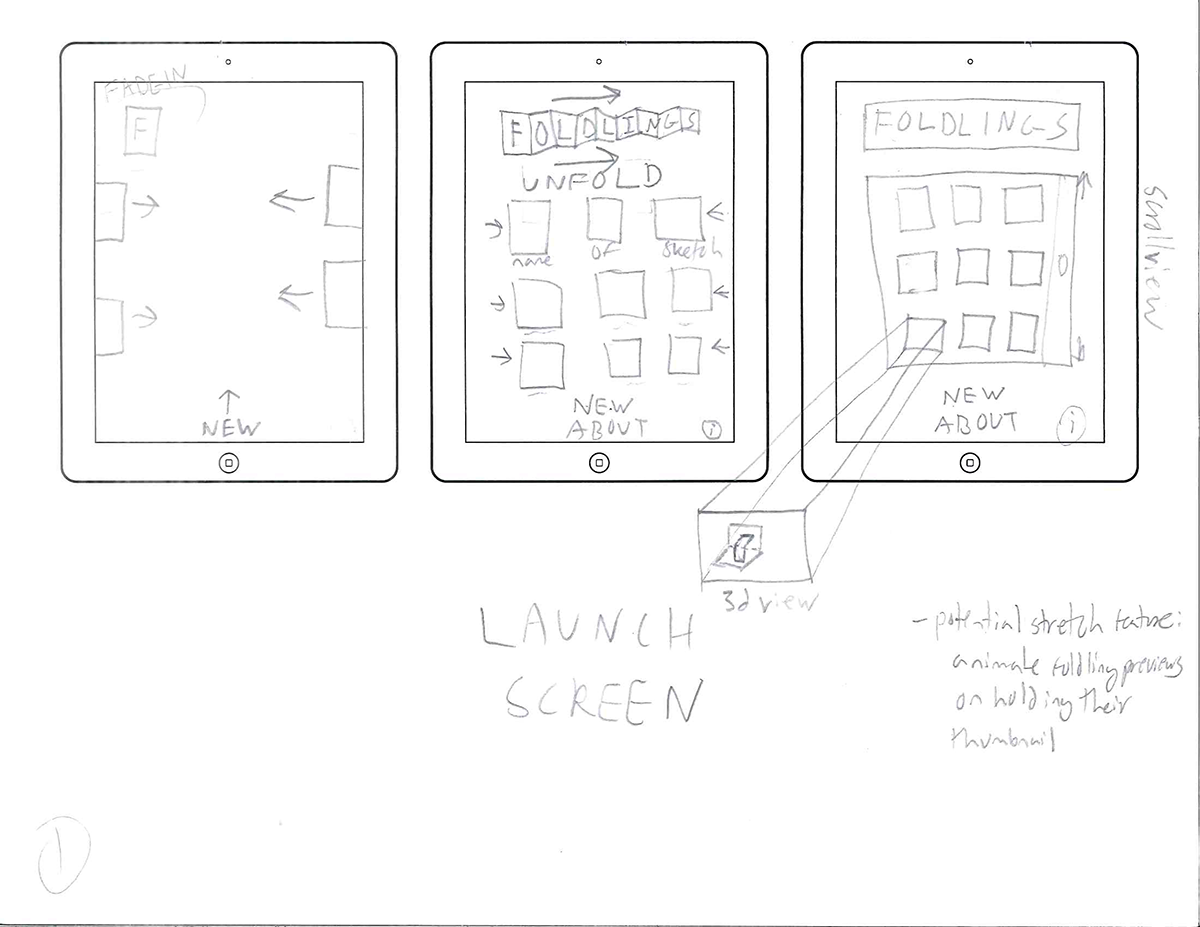
\includegraphics{figures/90_Appendix_UI_Mockups/001.png}
\caption{Initial mockups showing cards for saved sketches on the main
screen.}
\end{figure}

We started development in Fall 2014, as the final project for a course
on Computational Fabrication at Dartmouth. By December 2014, we had a
functional prototype of our popup card design software. Users could
create cuts and folds and fabricate them using a laser cutter. However,
in many ways our software was no better than manually creating cards. In
order to create a valid and beautiful design, users needed some prior
knowledge of the geometric constraints described in Chapter 3, section
\ref{constraints-on-fold-features} \ref{geometric-constraints},
\nameref{geometric-constraints}, on page
\pageref{geometric-constraints}. Performance problems also hampered
users' ability to create designs. Our goal was to improve both of these
aspects of Foldlings dramatically, to arrive at an intuitive and
functional tool. Paper mockups were an integral part of our design
process. We used these paper mockups to drive interface development, and
also to quickly get feedback from users before investing development
resources\footnote{See Appendix X: for samples of paper mockups we
  created during the design process}.

In arriving at our final design, we iterated through several potential
designs, each time getting feedback through informal user studies. We
made many changes to the toolset and experience based on feedback from
users. The final approach is ``feature-based'' --- in other words, the
user creates multiple cuts and folds in a single action, rather than
individually. These discrete logical units allow the user to design more
quickly, and to combine multiple different feature types to create
complex designs. A key advantage to this design over a less structured
approach is modularity. This is both an algorithmic and an interface
advantage: our algorithms benefit from collecting cuts and folds into
discrete logical units, and the user benefits from a faster and more
structured design process.

\begin{figure}[htbp]
\centering
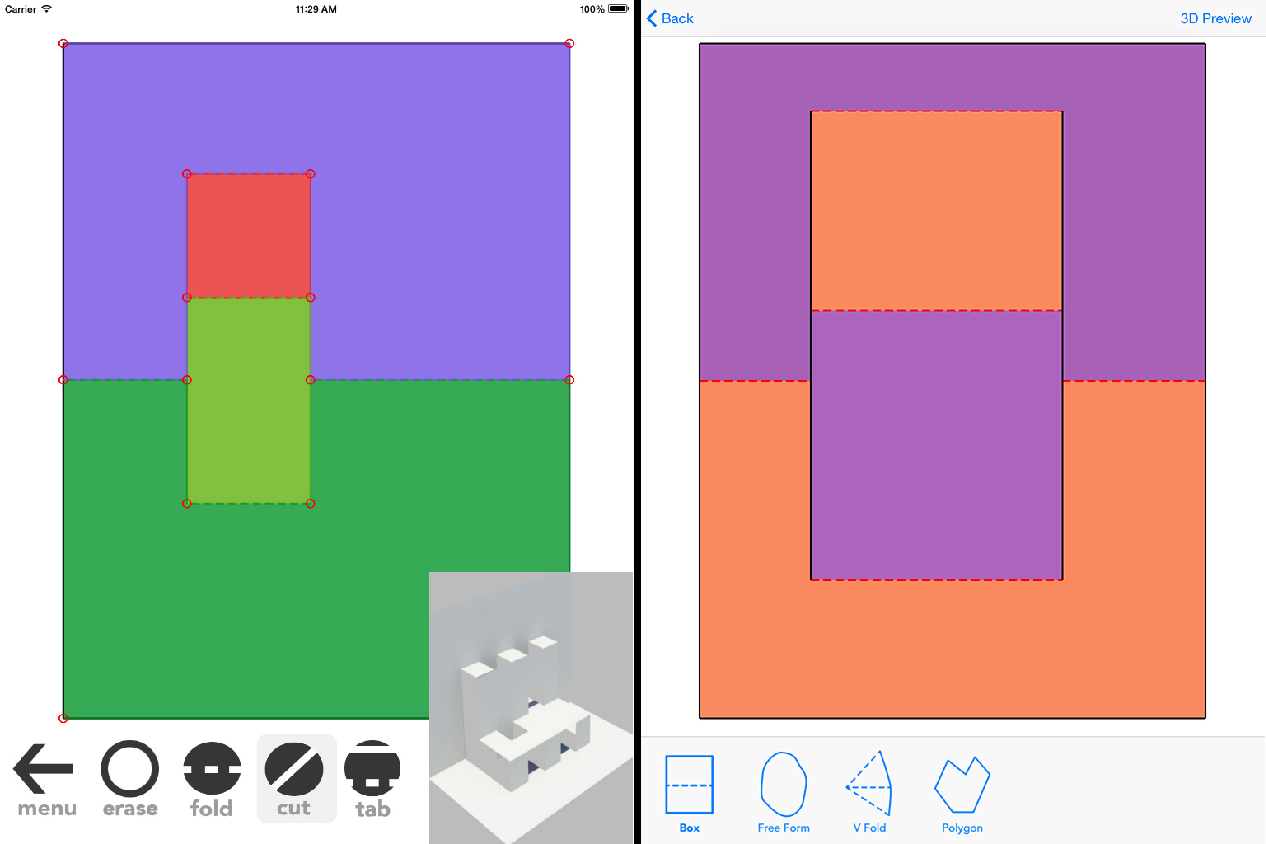
\includegraphics{figures/31_UI_Interface_Iteration/beforeafterinface.pdf}
\caption{Left: drawing interface as of December 2014. Right: drawing
interface as of August 2015.}
\end{figure}

Throughout the development process, we collected feedback through
informal user tests. One test we performed involved presenting a
partially-implemented version of our software to users. The majority of
buttons were functional --- erase, cut, fold, and and tab, but our
interface also contained buttons for unimplemented features. The primary
goals were to test whether our existing tools were useful and to collect
feedback on potential new features for Foldlings. When a user tapped a
button that we had not yet implemented, we asked them to describe how
they thought the tool would work, and talked with them about the
behavior the button represented.

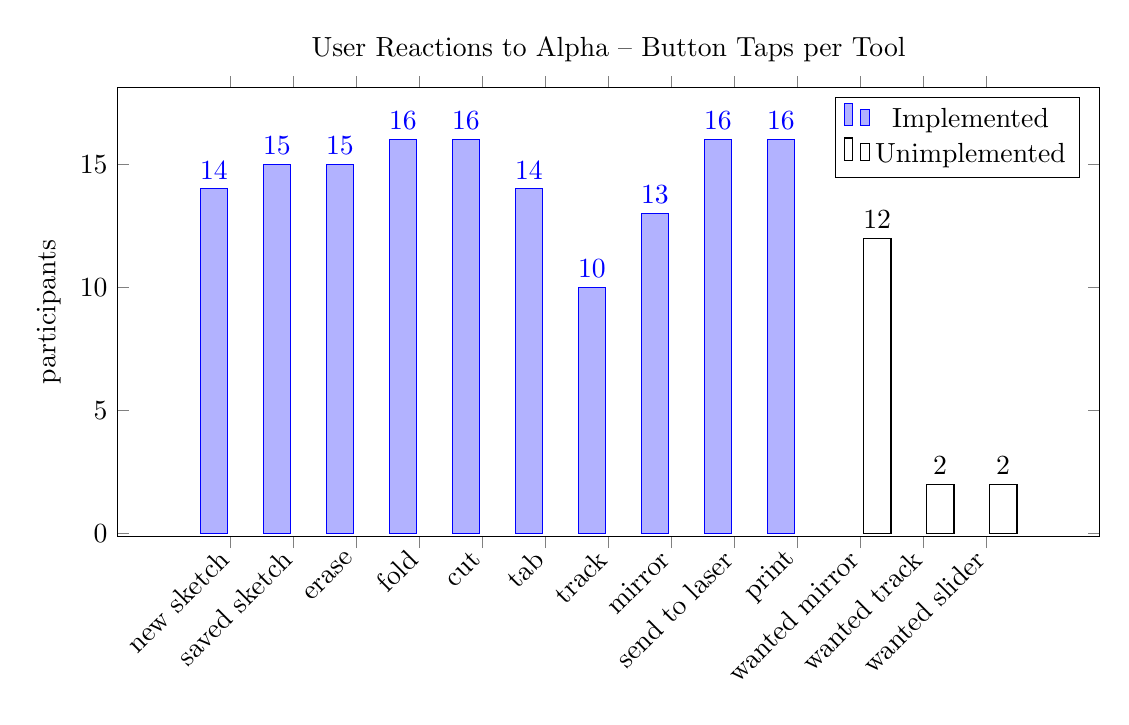
\begin{tikzpicture}
\begin{axis}[%
enlargelimits=0.15,
x=0.8cm,
title=User Reactions to Alpha -- Button Taps per Tool,
 symbolic x coords={new sketch,saved sketch,erase,fold,cut,tab,track,mirror,send to laser,print,wanted mirror,wanted track,wanted slider},
nodes near coords,
xtick={new sketch,saved sketch,erase,fold,cut,tab,track,mirror,send to laser,print,wanted mirror,wanted track,wanted slider},
ylabel style={align=center},
ylabel={participants},
x tick label style={rotate=45,anchor=east},
legend entries={Implemented, Unimplemented},
ybar]


\addplot coordinates {(new sketch,14)(saved sketch,15)(erase,15)(fold,16)(cut,16)(tab,14)(track,10)(mirror,13)(send to laser,16)(print,16)};
\addplot[color=black] coordinates {(wanted mirror,12)(wanted track,2)(wanted slider,2)};

\end{axis}
\end{tikzpicture}

In the graph above, the first ten labels indicate the number of
participants who tapped a button. The last three labels --- starting
with ``wanted mirror,'' show responses to unimplemented tools. To
calculate these numbers, we asked first users to describe what they
thought the button would do, and then gauged their reaction as we
described our vision for that tool. The tally represents a qualitative
measure of whether the user was enthusiastic about the feature or had a
more negative response. Some negative responses include confusion about
the tool's purpose and statements such as ``I don't think I would want
to use that.''

The unimeplemtneed tools were:

\begin{enumerate}
\def\labelenumi{\arabic{enumi}.}
\itemsep1pt\parskip0pt\parsep0pt
\item
  Mirror: a tool that would take an existing group of edges and reflect
  them about a fold in the sketch
\item
  Track: a tool that would create a cut in the sketch, and a second
  shape that would move within the cut, with folded tabs on the opposite
  side of the card. This tool required multiple pieces of paper.
\item
  Slider: a tool that would create a parallel set of cuts, making a
  ``pocket'' that a second shape would slide through. This tool required
  multiple pieces of paper.
\end{enumerate}

Each of these tools was inspired by features often found in
commercially-designed popup card and popup books
(\citet{birmingham1997pop}).

From this test, we learned that the track and slider tools were
confusing, and that novice users were generally not interested in
creating features that require multiple pieces of paper.

As users created sketches using our software, we also took notes on
their experience and collected suggestions for improvements. Although
only a small fraction of the features requested by users are implemented
in the final app, the feedback from these early user tests set us on the
path toward feature-based design. A common theme among the observation
in Table 2.1 is the difficulty in creating valid sketches and confusion
about the proposed track and slider tools.

\begin{longtable}[c]{@{}l@{}}
\caption{Observations of behavior from first user test.}\tabularnewline
\toprule
\begin{minipage}[b]{0.82\columnwidth}\raggedright\strut
Observations
\strut\end{minipage}\tabularnewline
\midrule
\endfirsthead
\toprule
\begin{minipage}[b]{0.82\columnwidth}\raggedright\strut
Observations
\strut\end{minipage}\tabularnewline
\midrule
\endhead
\begin{minipage}[t]{0.82\columnwidth}\raggedright\strut
made a cake using cuts \& tab, crashed on returning to sketch
\strut\end{minipage}\tabularnewline
\begin{minipage}[t]{0.82\columnwidth}\raggedright\strut
track and slider will need explanation; wanted to use non-horizontal
folds
\strut\end{minipage}\tabularnewline
\begin{minipage}[t]{0.82\columnwidth}\raggedright\strut
erased master fold, crashing at preview step
\strut\end{minipage}\tabularnewline
\begin{minipage}[t]{0.82\columnwidth}\raggedright\strut
made a cat with cuts
\strut\end{minipage}\tabularnewline
\begin{minipage}[t]{0.82\columnwidth}\raggedright\strut
momentary confusion getting back to sketch from 3D preview
\strut\end{minipage}\tabularnewline
\begin{minipage}[t]{0.82\columnwidth}\raggedright\strut
confused about concept of a laser cutter
\strut\end{minipage}\tabularnewline
\begin{minipage}[t]{0.82\columnwidth}\raggedright\strut
very frustrated by tools that aren't implemented yet
\strut\end{minipage}\tabularnewline
\begin{minipage}[t]{0.82\columnwidth}\raggedright\strut
confused by track \& slider
\strut\end{minipage}\tabularnewline
\begin{minipage}[t]{0.82\columnwidth}\raggedright\strut
needed heavy guidance; completely confused by track/slider
\strut\end{minipage}\tabularnewline
\begin{minipage}[t]{0.82\columnwidth}\raggedright\strut
fairly self-sufficient after tools were explained, made a house, moved
slowly, waiting for planes to calculate
\strut\end{minipage}\tabularnewline
\bottomrule
\end{longtable}

A common theme among the feature requests was a desire for a more
complete tutorial and explanation of tools. Features only appear once in
Table 2.2, even if they were requested by multiple people. The
most-requested feature was an interactive tutorial, requested by 4 (of
16) users. In the final version of our software, we display short
example videos when users use a tool for the first time. See Chapter 2,
section \ref{tool-interactions} \ref{tutorial} \nameref{tutorial} on
page \pageref{tutorial} for more discussion. These tutorials allow users
to quickly get started quickly with minimal interruptions.

\begin{longtable}[c]{@{}l@{}}
\caption{Feedback from first user test.}\tabularnewline
\toprule
\begin{minipage}[b]{0.82\columnwidth}\raggedright\strut
Feature Requests
\strut\end{minipage}\tabularnewline
\midrule
\endfirsthead
\toprule
\begin{minipage}[b]{0.82\columnwidth}\raggedright\strut
Feature Requests
\strut\end{minipage}\tabularnewline
\midrule
\endhead
\begin{minipage}[t]{0.82\columnwidth}\raggedright\strut
option to reverse all folds
\strut\end{minipage}\tabularnewline
\begin{minipage}[t]{0.82\columnwidth}\raggedright\strut
draw over existing fold with tab tool
\strut\end{minipage}\tabularnewline
\begin{minipage}[t]{0.82\columnwidth}\raggedright\strut
non-horizontal folds
\strut\end{minipage}\tabularnewline
\begin{minipage}[t]{0.82\columnwidth}\raggedright\strut
fold by pinching
\strut\end{minipage}\tabularnewline
\begin{minipage}[t]{0.82\columnwidth}\raggedright\strut
rename sketches
\strut\end{minipage}\tabularnewline
\begin{minipage}[t]{0.82\columnwidth}\raggedright\strut
delete sketches
\strut\end{minipage}\tabularnewline
\begin{minipage}[t]{0.82\columnwidth}\raggedright\strut
orthographic views
\strut\end{minipage}\tabularnewline
\begin{minipage}[t]{0.82\columnwidth}\raggedright\strut
long press to view information about tool
\strut\end{minipage}\tabularnewline
\begin{minipage}[t]{0.82\columnwidth}\raggedright\strut
reorder sketches on main screen
\strut\end{minipage}\tabularnewline
\begin{minipage}[t]{0.82\columnwidth}\raggedright\strut
interactive tutorial
\strut\end{minipage}\tabularnewline
\begin{minipage}[t]{0.82\columnwidth}\raggedright\strut
more snapping/validity guidance
\strut\end{minipage}\tabularnewline
\bottomrule
\end{longtable}
